\documentclass[10pt]{article}
\usepackage[utf8]{inputenc}
\usepackage[czech]{babel}
\usepackage{a4wide}
\usepackage{amsmath}
\usepackage{graphicx}

\usepackage{bigstrut}
\usepackage{multirow}


\newcommand{\labtitle}[4]{
	\begin{titlepage}
		\begin{center}
			\mbox{} \\[4cm]
			{\huge {#1}} \\[2cm]
			{\Large #2}  % \\[.2cm]
			{\large #3 } \\[.7cm]
			{\normalsize měřeno #4}
		\end{center}
	\end{titlepage}
}

\title{Ohyb a interference světla optickou mřížkou}
\author{Tomáš Maršálek}
\date{10. října 2011}

\begin{document}
% --- title start --- %
 \labtitle{Ohyb a interference světla optickou mřížkou}
 {Tomáš Maršálek}
 {(A10B0632P)}
 {10.\,října 2011}
% --- title end --- %

\section{Měřící potřeby a přístroje}
spektrometr, optická mřížka, sodíková výbojka, Balmerova lampa
%% WTF %% \section{Pracovní úkol}

\section{Naměřené hodnoty}
\subsection{Sodíková výbojka}
\begin{tabular}[b]{|c|c|c|c|c|c|c|}
	\hline
	\bigstrut
	řád & $\alpha^\prime~[^\circ]$ & $\beta~[^\circ]$ & 
	$\alpha^{\prime\prime} = 360 - \beta~[^\circ]$ &
	$\alpha = \frac{\alpha^\prime + \alpha^{\prime\prime}}{2}~[^\circ]$ &
	$\sin(\alpha)$ & d [nm] \\
	\hline
	1 & 20.8 & 339.0 & 21.0 & 20.9 & 0.36 & 1\,636.9 \\
	2 & 45.4 & 314.5 & 45.5 & 45.5 & 0.71 & 1\,660.0 \\
	\hline
\end{tabular}

\subsection{Balmerova lampa}
\begin{footnotesize}
\begin{tabular}[b]{|c|l|c|c|c|c|c|c|c|c|}
	\hline
	\bigstrut
řád & barva & $\alpha^{\prime}~[^\circ]$ & $\beta^{\prime}~[^\circ]$ 
& $\alpha^{\prime\prime} = 360 - \beta ~[^\circ]$ & 
$\alpha = \frac{\alpha^{\prime} + \alpha^{\prime\prime}}{2}~[^\circ]$ 
& $\sin(\alpha)$ & $\lambda~[nm]$ & $n$ & $R~[cm^{-1}]$ \\
\hline

\multirow{5}{*}{1} 
& fialová1    & 14.4 & 345.6 & 14.4 & 14.4 & 0.25 & 409.97 & 6 & 109\,765.393\,1 \\
& fialová2    & 15.2 & 344.6 & 15.4 & 15.3 & 0.26 & 434.99 & 5 & 109\,470.403\,0 \\
& modrozelená & 17.0 & 342.8 & 17.2 & 17.1 & 0.29 & 484.73 & 4 & 110\,027.914\,7 \\
& oranžová    & 21.9 & 338.0 & 22.0 & 21.9 & 0.37 & 616.20 & - & -           \\
& červená     & 23.3 & 336.5 & 23.5 & 23.4 & 0.40 & 654.70 & 3 & 109\,974.319\,9 \\
\hline

\multirow{5}{*}{2} 
& fialová1    & -    & -     & -    & -    & -    & -      & 6 & -           \\
& fialová2    & 31.7 & 328.3 & 31.7 & 31.7 & 0.53 & 433.12 & 5 & 109\,944.234\,2 \\
& modrozelená & 36.0 & 324.0 & 36.0 & 36.0 & 0.59 & 484.48 & 4 & 110\,083.210\,5 \\
& oranžová    & 48.1 & -     & -    & 48.1 & 0.74 & 613.50 & - & -           \\
& červená     & 52.5 & 307.5 & 52.5 & 52.5 & 0.79 & 653.92 & 3 & 110\,104.960\,6 \\
\hline

\multirow{2}{*}{3} 
& fialová2    & -    & - & - & -    & -    & -      & 5 & -           \\
& modrozelená & 61.9 & - & - & 61.9 & 0.88 & 484.73 & 4 & 110\,027.180\,0 \\
	\hline
\end{tabular}
\end{footnotesize}

\section{Výpočty}
Podmínka pro maximum intenzity ve směru podle úhlu $\alpha$. $d$ je mřížková
konstanta, $k$ je řád a $\lambda$ vlnová délka.
\begin{equation}
d \sin \alpha = k \lambda
\label{podminka_maxima}
\end{equation}

Balmerův vztah, kde $R$ je Rydbergova konstanta, $1/\lambda_n$ vlnočet
a~$n$ kvantové číslo podle barvy emisní čáry.
\begin{equation}
\frac{1}{\lambda_n} = R \left(\frac{1}{2^2} - \frac{1}{n^2}\right)
\label{balmer}
\end{equation}

\subsection{Sodíková výbojka}
Z rovnice \eqref{podminka_maxima} získáme hodnoty $d$ uvedené výše 
v~tabulce. Vlnová délka žlutého světla sodíkové výbojky je 589.3 nm.
Průměrná hodnota mřížkové konstanty je $\lambda = 1\,648.5$~nm.
Počet vrypů na jednotku je převrácená hodnota $d$, pro použitou optickou
mřížku vychází 606 vrypů na 1~mm.

\subsection{Balmerova lampa}
Mřížkovou konstantu známe z předchozího měření, pomocí vztahu 
\eqref{podminka_maxima} zjistíme vlnové délky pro jednotlivé barvy.
Z rovnice \eqref{balmer} pak pro každou barvu vypočteme 
Rydbergovu konstantu. Její průměrná hodnota vyšla $R = 109\,924.701\,9~cm^{-1}$.

%% plot
\begin{center}
\includegraphics[width=10cm,angle=270]{lab1.eps}
\end{center}

\section{Závěr}
Některé hodnoty nebyly naměřeny, protože jejich příslušné barvy nebyly
při měření zřetelné (fialová1 a několik barev při vyšším řádu).
Výsledkem prvního měření je počet vrypů na jednotu délky, odpovídá
{\boldmath $606$ }vrypům {\bf na 1~mm }. Z druhého úkolu byla vypočtena hodnota 
Rydbergovy konstanty {\boldmath $R = 109\,924.701\,9\pm197.921\,4~cm^{-1}$}, 
což odpovídá tabulkové hodnotě $109\,737.314\,3~cm^{-1}$ . Rozdíl je menší
než jedna směrodatná odchylka.





\end{document}
